%!TEX root = ../Main.tex

\section{Methodology and Data}
\subsection{Methodology: Linear Regression and HAR-RV model}
\begin{itemize}\itemsep0pt
\item Reg1: without VIX
\begin{itemize}\itemsep0pt
\item Reg1a: regress realized volatility on historic volatility using simple linear regression
\item Reg1b: regress realized volatility on historic volatility using HAR-RV model
\end{itemize}
\item Reg2: with VIX
\begin{itemize}
\item Reg2b: regress realized volatility on historic volatility using simple linear regression
\item Reg2b: regress realized volatility on historic volatility using HAR-RV model
\end{itemize}
\end{itemize}
%
\begin{flalign}
&\sigma_{t,x}^{RV} = \alpha_{x,t} + \beta_{x,t}^{HV} \sigma_{x,t}^{HV}\\
&\sigma_{x,t}^{RV} = \alpha_{x,t} + \beta_{x,t}^{HV,d} \sigma_{x,t}^{HV,d} + \beta_{x,t}^{HV,w} \sigma_{x,t}^{HV,w} + \beta_{x,t}^{HV,m} \sigma_{x,t}^{HV,m}\\
&\sigma_{x,t}^{RV} = \alpha_{x,t} + \beta_{x,t}^{HV} \sigma_{x,t}^{HV} + \beta_{x,t}^{VIX} + \sigma^{VIX}_{x,t}\\
&\sigma_{x,t}^{RV} = \alpha_{x,t} + \beta_{x,t}^{HV,d} \sigma_{x,t}^{HV,d} + \beta_{x,t}^{HV,w} \sigma_{x,t}^{HV,w} + \beta_{x,t}^{HV,m} \sigma_{x,t}^{HV,m} + \beta_{x,t}^{VIX} + \sigma^{VIX}_{x,t}
\end{flalign}

\subsection{Data and Calculation of Input Factors}
\begin{figure}[!htbp]
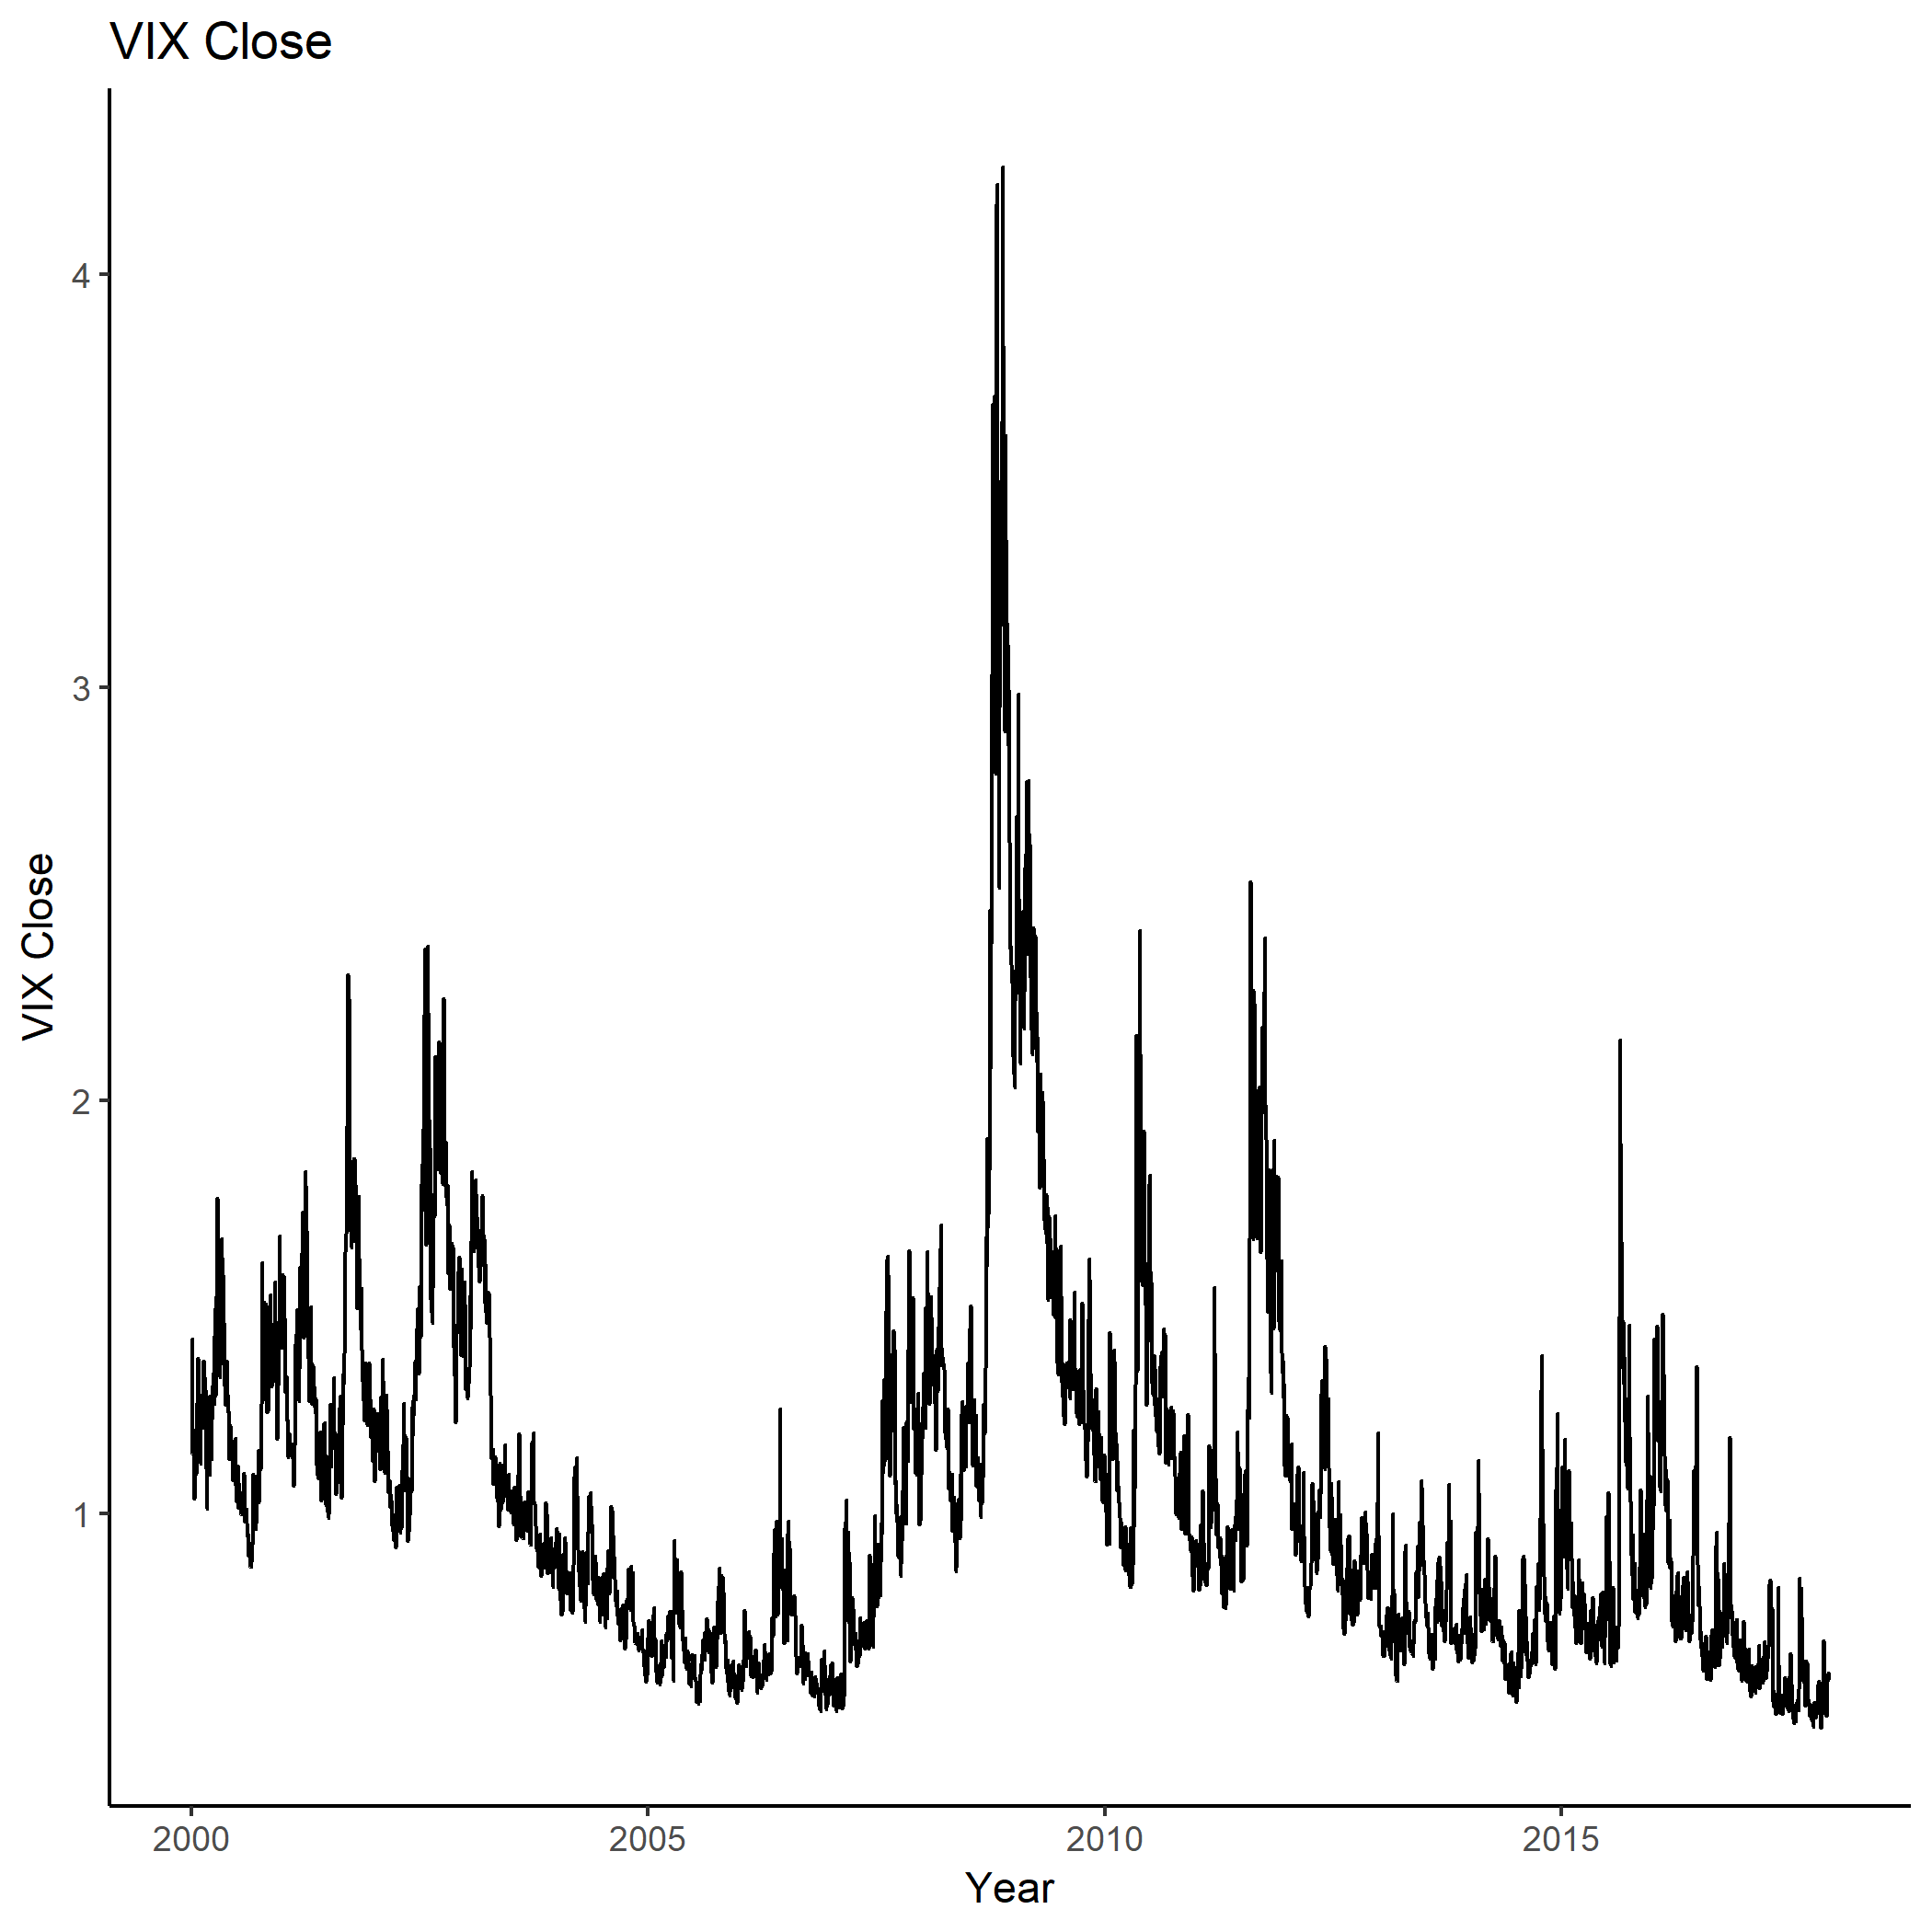
\includegraphics[width=16cm, height=8cm]{pictures/vix.png}
\end{figure}
%
\begin{figure}[!htbp]
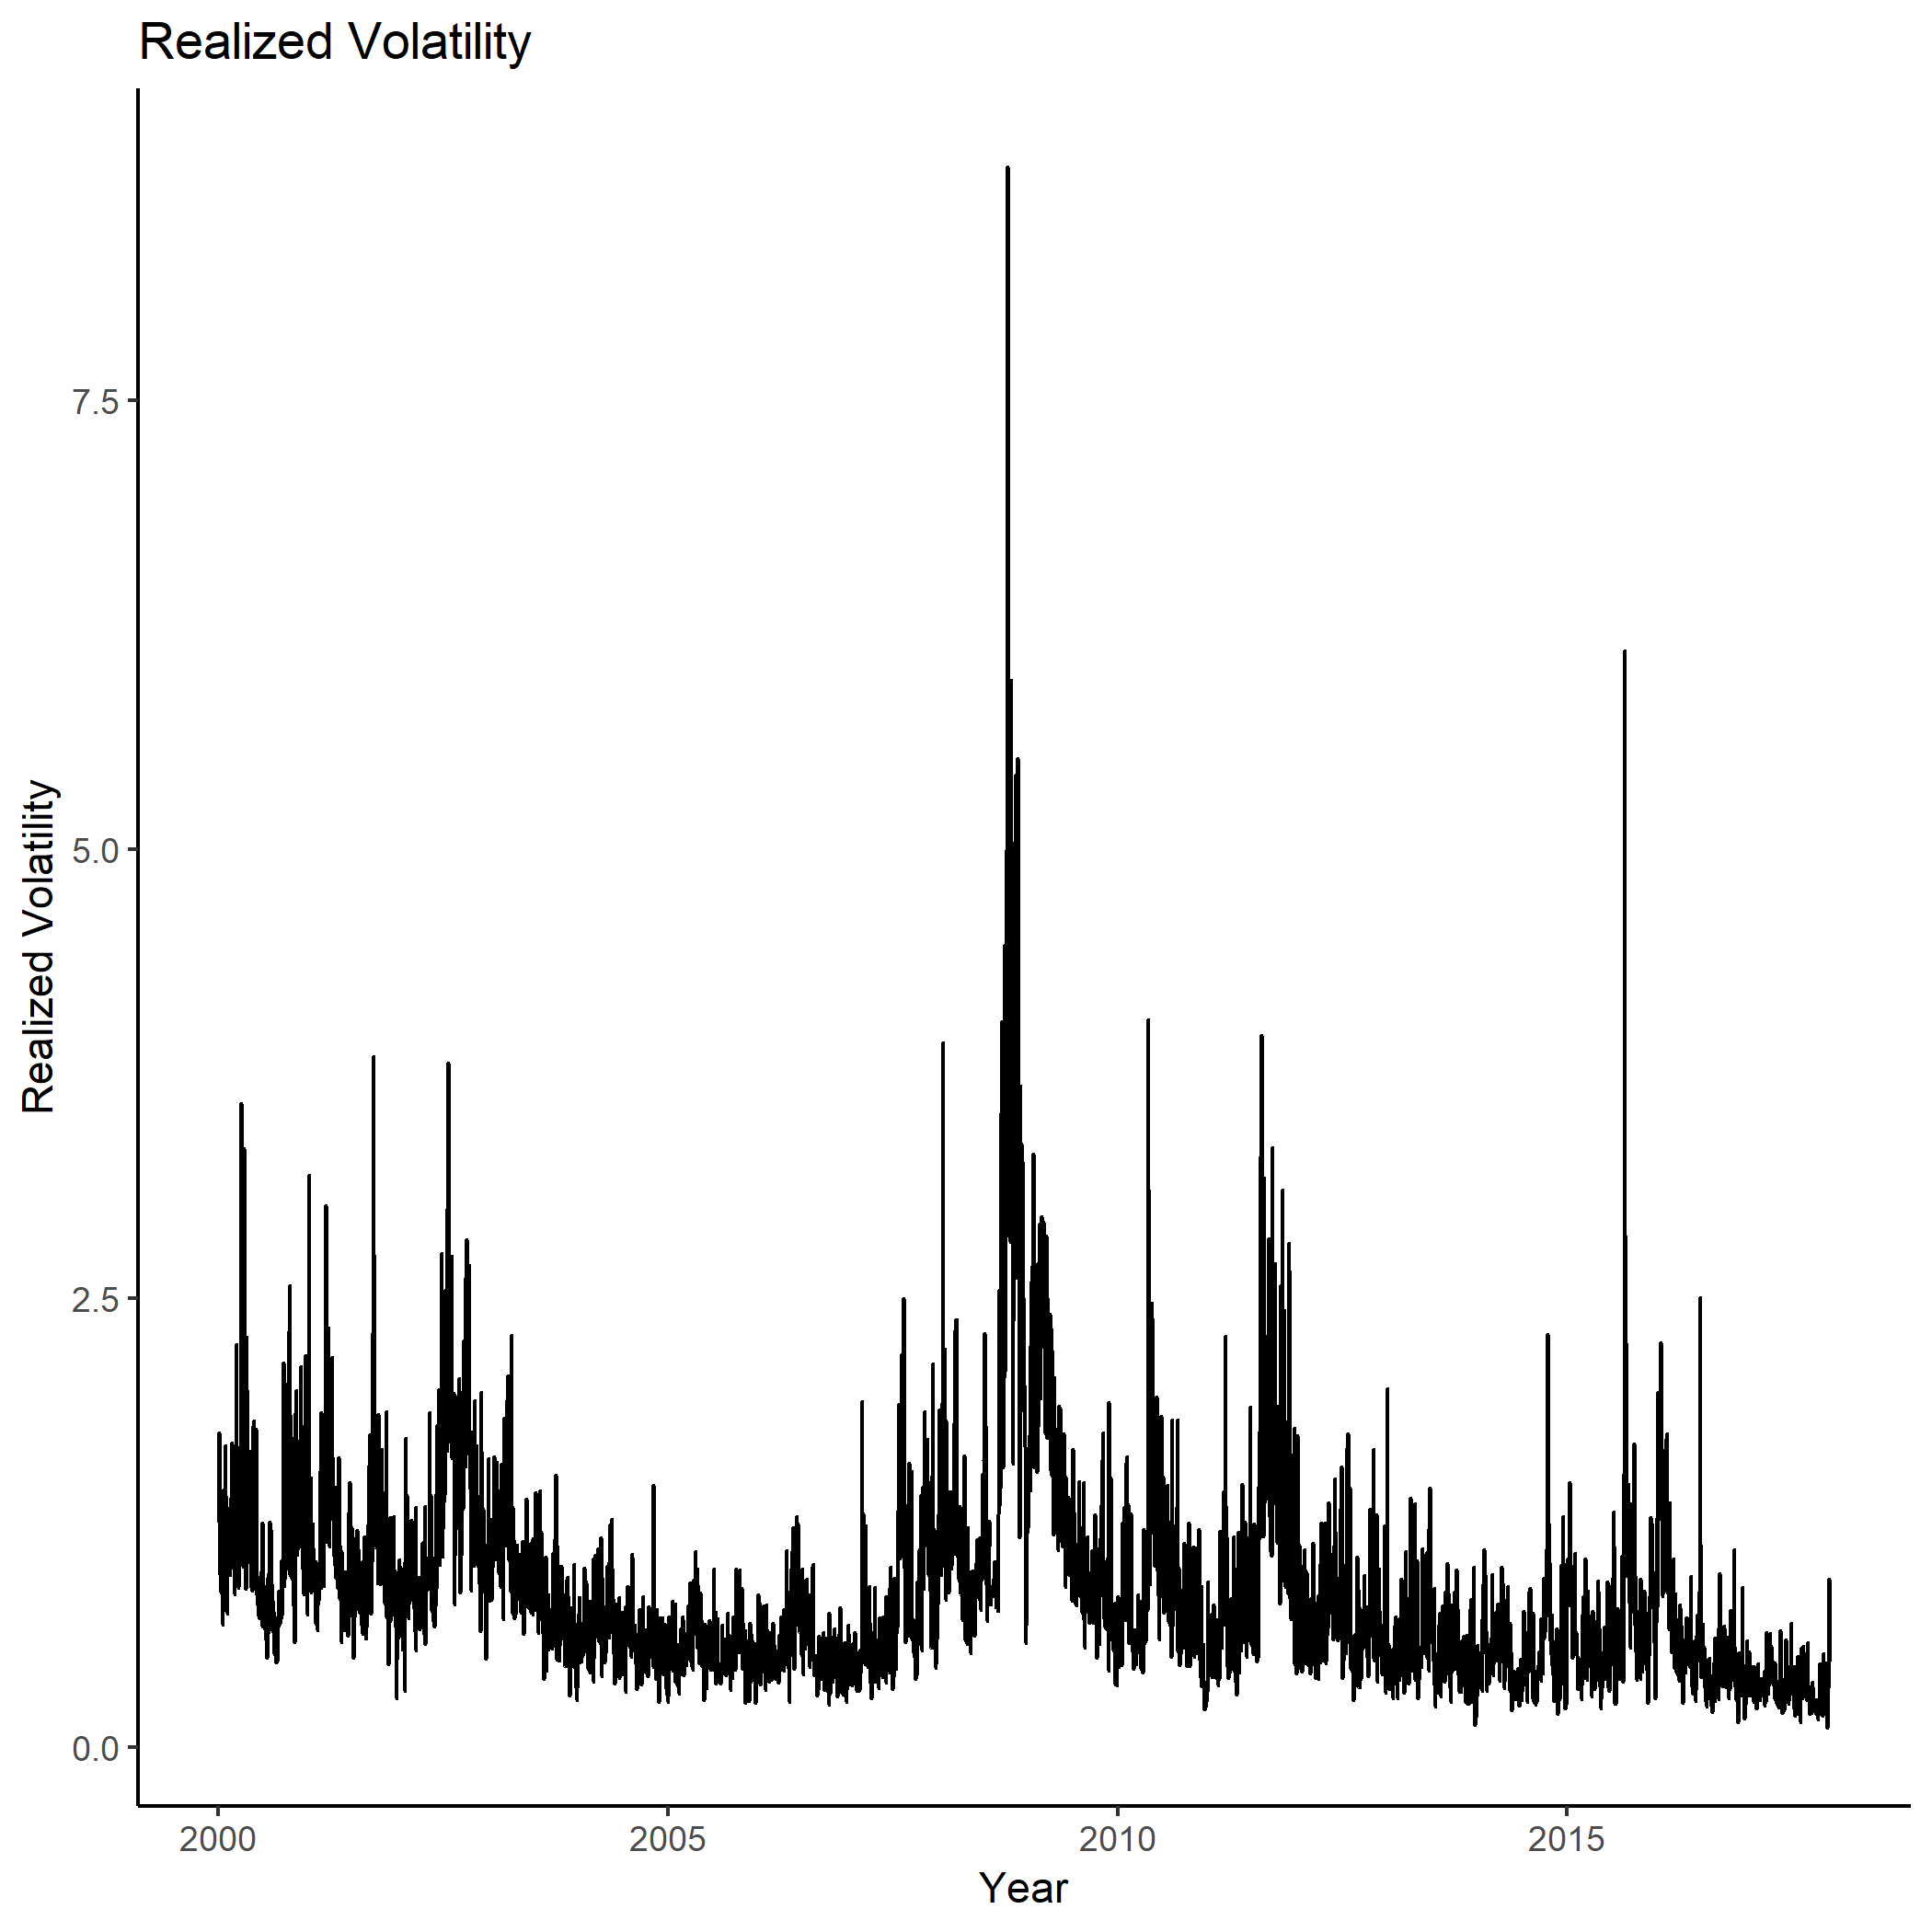
\includegraphics[width=16cm, height=8cm]{pictures/vol.png}
\end{figure}
%
\begin{figure}[!htbp]
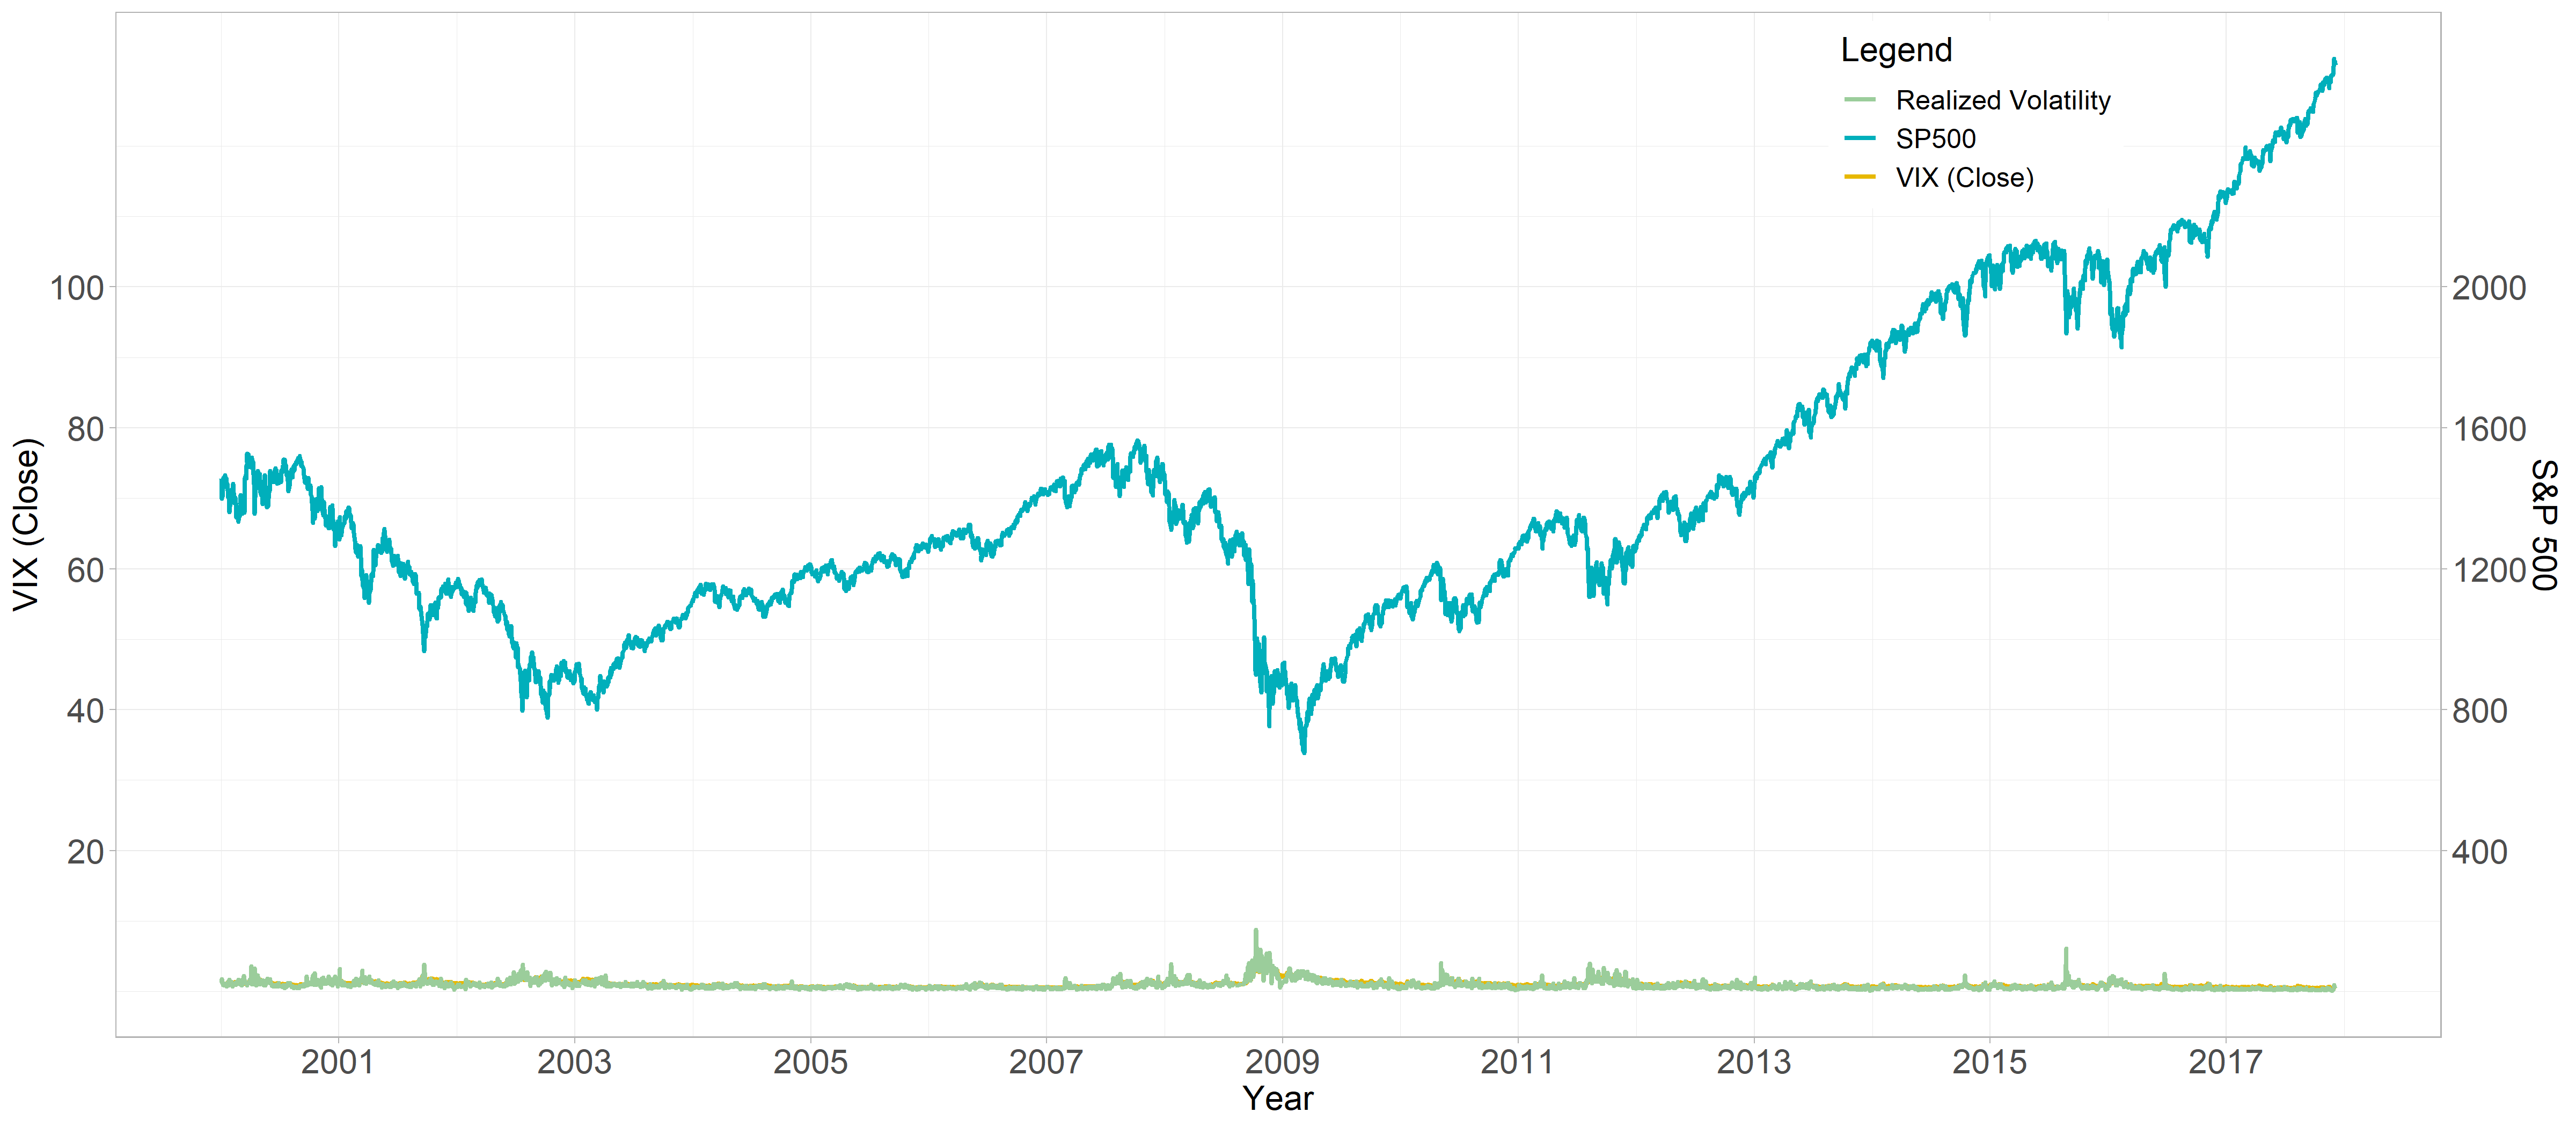
\includegraphics[width=16cm, height=8cm]{pictures/SPandVolandViX.png}
\end{figure}

%\input{pictures/var.png}
%\input{pictures/vix.png}
\begin{itemize}\itemsep0pt
\item S\&P 500 index data on daily basis
\item sampling period: 2000 - 2018
\item realized volatility: daily realized volatility of S\&P 500, calculated using 5 minute returns, retrieved from \citeauthor{heber2009}
\item model-free implied volatility: VIX index data
\item historic volatility: lagged realized volatility, for HAR-RV model use the average over the time period used to forecast
\end{itemize}
